\documentclass{article}

\usepackage[margin=.75in]{geometry}
\usepackage{listings}
\usepackage{amsmath}
\usepackage[hidelinks]{hyperref}
\usepackage{graphicx}

\lstset{
    basicstyle=\ttfamily,
    mathescape
}

\author{Damien Prieur}
\title{Homework 4 \\ CS 457}
\date{}

\begin{document}

\maketitle

\section*{Question 1}
You are given a red-black tree $T$ with 15 internal nodes (nodes that hold key values)
that form a \emph{full} binary tree of height 3 (i.e., a full binary tree of height 4 if you include
the NIL leaves). Can you assign colors to the nodes so that a call to \textsc{RB-Insert}($T,z$) for
\emph{any} new key value $z.key$ will cause \textsc{RB-Insert-Fixup}($T,z$) to change the color of the
root to red before switching it back to black? The initial assignment of colors needs to obey the
red-black properties. If such a color assignment exists, then provide a sequence of 15 numbers whose
insertion (in that order) would lead to such a tree, along with a figure of the resulting tree. If not,
then explain why such an assignment cannot exist, using the fact that the tree needs to satisfy the
red-black properties. You can use the applet \url{https://www.cs.usfca.edu/~galles/visualization/RedBlack.html}
and read through Chapter 13 from your textbook if you would like to better understand how red-black trees work.

\begin{figure}[h]
    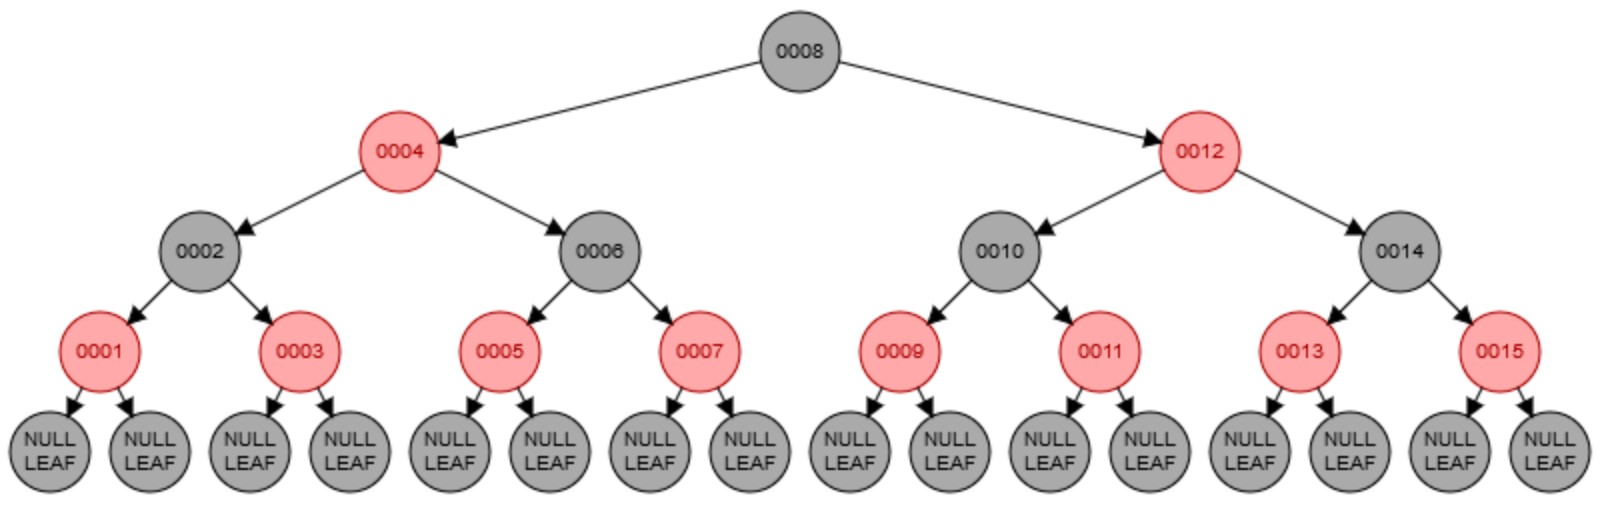
\includegraphics[width=\linewidth]{full_RB_tree.jpg}
\end{figure}

Insertion order:
8,4,12,2,14,6,10,1,3,5,7,9,11,13,15

\section*{Question 2}
A full $k$-ary tree is a (rooted) tree whose nodes either have exactly $k$ children
(internal nodes) or have no children (leaves). \emph{Using induction}, formally prove that every full
$k$-ary tree that has $x$ internal nodes has exactly $kx+1$ nodes in total. Note that for full
\emph{binary} trees, i.e., when $k=2$, this would imply that the total number of nodes is $2x+1$,
which would verify what Cameron suggested in class (that the total number of nodes of full binary
trees is always odd).
\newline
\newline
\indent For the base case we can look at a tree with one node. This tree has $0$ internal nodes so we have $k\cdot 0 + 1=1$ node in our tree.
For our inductive step we can look at how we can add nodes to increase our internal node count.
We can select any leaf, we can't choose an internal node to add nodes to as they would become over-populated.
With the leaf we must add k leaves so that our tree is still complete.
Doing so causes our chosen leaf to become an internal node and adds k new nodes.
Assume that any $k$-ary tree that has $n$ internal nodes has exactly $kx+1$ nodes in total.
To show that this holds for $n+1$ internal nodes we begin with our assumption for n.
$$Total \; nodes = kn+1$$
Based on the argument above selecting a leaf to add new nodes to increases our internal node count by $1$, $n'=n+1$, and increases our total node count by $k$, $Total \; nodes'=kn+1+k$.
Rearranging these terms we get
$$Total \; nodes' = k(n+1)+1 = kn'+1$$
Which agrees with our original equation for n+1.


\section*{Question 3}
Using proof by induction, show that there are at most $\lceil n/2^{h+1}\rceil$
nodes of height $h$ in any $n$-element heap. Make sure to clearly state your base case and your
inductive step arguments. Also note that you need to prove the aforementioned upper bound for the
number of nodes of height $h$ for \emph{every} value of $n$ and \emph{every} $n$-element heap.
\newline
\newline


We can solve this problem using induction on the height for a heap of size n.
For our base case we will look at $h = 0$.
We know that the number of nodes at height $0$ is equal to the number of leaves.
In a heap the number of leaves is $\lceil \frac{n}{2} \rceil$
$$ \lceil \frac{n}{2} \rceil <= \lceil n/2^{0+1}\rceil $$
In fact the number of leaves is exactly described by the equation we are trying to show.
\\
Now for the inductive step, assume it works for height $h$ show that it holds for $h+1$.
There are two cases, one in which the number of nodes in $h$ is even and one where the number of nodes in $h$ is odd.
For the even case then each pair of nodes has one parent each since we are a heap, so the number of nodes becomes
$$\frac{\text{node count}}{2}$$
While for the odd case we will have the same logic expect for the node with no pair it will still have one parent, this gives us a node count of
$$\frac{\text{node count} - 1}{2} + 1 = \lceil \frac{\text{node count}}{2} \rceil$$
So we can combine these two cases with $h+1$ having
$$\lceil \frac{\text{node count}}{2} \rceil$$
nodes where node count is the number of nodes in height $h$
Using our assumption we have that
$$\text{node count} <= \lceil n/2^{h+1}\rceil$$
We get that at height $h+1$ we have
$$\lceil \frac{\lceil n/2^{h+1}\rceil}{2} \rceil \ge \lceil \frac{n}{2^{(h+1)+1}} \rceil$$
Which matches our equation for height $h+1$ as we would get
$$\lceil n/2^{(h+1)+1}\rceil $$

With our base case solved we have shown this is true for all heights in any heap of size $n$

\section*{Question 4}
You start a new tech business and you reach the point where you have offices both in the
east coast and in the west coast. There are different operating costs involved in running your business
in each location, so you may need to move back and forth across the coasts in order to minimize the total
costs. However, there are moving costs involved in traveling from one coast to the other which complicate
your problem. More formally, for each month $i=1,\dots, n$ you have an operating cost $e_i$ associated
with running your business in the east coast during that month and an operating cost $w_i$ for the west coast.
You can begin working in either coast, but after any subsequent travel from one coast to another you suffer
a fixed travel cost of $c$. Given input $\{e_1,\dots, e_n\}$, $\{w_1,\dots, w_n\}$, and $c$, provide a $O(n)$
time algorithm that outputs a plan defining which coast you will work from each month, and minimizes your
total cost (operating costs plus travel costs).
\newline
\newline

For example, if the number of months was $n=5$, a possible plan could be to work from the east coast during
the first two months, then spend the next two months working from the west coast, and return to the east coast
for the fifth and final month. The total cost in this case would be $e_1+e_2+c+ w_3+w_4+c +e_5$, where the
two costs of $c$ are due to the change of coast. Provide detailed pseudocode for your proposed algorithm, as
well as an explanation regarding why it works and why its running time is indeed $O(n)$.

We find the solution by solving two subproblems, one for the best way to end on the east coast for month i, and the other being the same but for the west coast.
With knowledge of the optimal solution for the subproblem we can trivially find the solution to the parent problem.
Compare the cost of staying on the coast you are on to switching from the other coast.
Once you repeat and reach month n compare the two values and select the one with lower cost.
To create the path you can keep track as you go what the path is to the current cost so that it can be returned at the end.
\newline
\newline
The psuedocode is all on it's own page
\newline
\newline

We can see that is algorithm is $O(n)$ as we iterate over the list of the months while doing constant amounts of work.

\pagebreak
\begin{lstlisting}
function (eastCoast, westCoast, c, n){

    //lists of n elements
    bE = [] //best cost ending on East coast for element i
    bW = [] //best cost ending on West coast for element i

    bEPath = []
    bWPath = []

    //Start on the respective coasts
    bE[0] = eastCoast[0]
    bW[0] = westCoast[0]

    bEPath[0] = "e"
    bWPath[0] = "w"

    for (i = 1; i < n ; i ++) {
        // find next east coast ending
        cost = bE[i-1]
        if( cost < (bW[i-1] + c) ){
            // Stay on east coast
            bE[i] = bE[i-1] + eastCoast[i]

        }else{
            // Switch from west coast
            bE[i] = bW[i-1] + c + eastCoast[i]

            //Copy existing path to get to West coast
            bEPath = bWPath
        }
        bEPath.append("E")

        // find next west coast ending
        cost = bW[i-1]
        if( cost < (bE[i-1] + c) ){
            // Stay on West coast
            bW[i] = bW[i-1] + westCoast[i]
        }else{
            // Switch from east coast
            bW[i] = bE[i-1] + c + westCoast[i]

            //Copy existing path to get to West coast
            bWPath = bEPath
        }
        bWPath.append("w")
    }

    if(bE[n-1] < bW[n-1]){
        return bEPath;
    }
    return bWPath;
}

\end{lstlisting}




\section*{Question 5}
You are planning to attend a music and arts festival that hosts multiple events that
you are interested in, but many of these events may (partially) overlap. Assume that you get some value
$v_i$ from attending an event $i$, but you get this value only if you are there for the whole duration
of the event; you get no value if you have to miss part of it. Given such a set of events, $E$, your
goal is to choose a non-overlapping set of events, $E'\subseteq E$, to attend, aiming to maximize your
total value. More formally, for each event $i\in E$ you have a start time $s_i$ and a finish time $f_i$ and
you want to design an algorithm that runs in time $O(n\log n)$, where $n$ is the total number of events,
and the output of the algorithm is a set $E'\subseteq E$ such that for any two events $i,j\in E'$ we have
$f_i\leq s_j$ or $f_j \leq s_i$ (no overlap) and the total value $\sum_{i\in E'} v_i$ is maximized. Provide
detailed pseudocode for your proposed algorithm (you can use sorting as a subroutine), as well as an explanation
regarding why it works and why its running time is indeed $O(n\log n)$.
\newline
\newline

First we can start by sorting the inputs by their end times so that it is easy to make comparisons for overlapping.
Then we can approach this problem similarly to the other problem, find the optimal solution up to each event but it doesn't need to include the event.
For the next event we can either choose to include it or not.
We include it if the sum of the optimal values up to the previous non-overlapping event is greater than the value of the largest overlapping event.
We can find the previous overlapping event by looking if the previous element overlaps with the current element.
To find the previous nonoverlapping element we can use binary search to find the element that exists where the start time of our event lives.
At the end we can compare the total values and the optimal solution.
For each optimal solution we can keep the set of events that are chosen in a list to be used for future calculations or returned as the final set.
\newline
\newline
The psuedocode is all on it's own page
\newline
\newline
We can see that this is $O(n\log{n})$ as we first sort which takes $O(n\log{n})$ then we iterate over the list of events.
While iterating we do constant work and preform a binary search which also takes $O(n\log{n})$.
Finally creating the optimal subset iterates over a list of at most length $n$ so that part is $O(n)$.
Overall this algorithm is $O(n\log{n})$

\pagebreak
\begin{lstlisting}

//helper functions

// e1 ends before e2
function overlapping(e1, e2){
    return e1.endTime > e2.startTime
}

function eventSchedule(events){
    // events is a list of events.
    // an event contains the starting time under "startTime"
    // an end time under "endTime"
    // and a value under "value"

    // want this just so that i don't have to deal with multiple lists while sorting

    // sort events by their end times
    events.sort(key="endTime")

    bValue = [] // list of best values by attending events up to and including event i

    // used to create set at the end
    parent = [] // holds index of "parent" previous element that we are chaining off of
    eventUsed = [] // booleans that say if an event is used in the optimal solution

    bValue[0] = events[0].value

    for (i=1; i < len(events); i++){

        // returns index of element
        // returns -1 if there are no previous nonoverlapping elements
        prevNonoverLapping = binarySearch(list=events, item=event[i].startTime,
                                          key="endTime", start=0, end=i)

        // we are the start of possibilities
        if(prevNonoverLapping == -1){
            bValue[i] = events[i].value
            parent = Null
            eventUsed = True
        }else{
            bValue[i] = bValue[prevNonoverLapping] + events[i].value
        }

        if(bValue[i] < bValue[i-1]){
            // skipping this event is worth it
            bValue[i] = bValue[i-1]
            parent[i] = i-1
            eventUsed = False
        }else if(prevNonoverLapping != -1){
            //if we are not the beginning of a new sequence

            // set some values to print path later
            parent[i] = prevNonoverLapping
            eventUsed = True
        }
    }

    optEvents = [] // set of events to go to

    while( i != Null){
        if(eventUsed[i]){
            optEvents.append(events[i])
        }
        i = parent[i]
    }

    return optEvents
}

\end{lstlisting}

\end{document}
